\selectlanguage{french}
\appendice{Comment la biodiversité s'installe en territoires isolés}
\label{annI}
\addtocounter{chapter}{1}
\setcounter{equation}{0}

% [Cette page est facultative; l’éliminer si elle n’est pas utilisée. Une annexe est jointe lorsqu’une information pertinente (tableau, figure ou autre) risque de nuire à la compréhension du texte principal ou encore de l’alourdir inutilement. Les annexes portent un titre (même mise en page que les chapitres) et sont numérotées en chiffres romains majuscules, s’il y en a plus d’une. On y fait référence dans le texte principal par la mention « voir ». Ex. : (voir annexe I).]


L'article qui suit est le fruit de ma recontre avec Philippe Etchécopar, un des membres du comité éditorial du journal \emph{Accro$\alpha$mth}.
Ce journal de vulgarisation mathématique est destiné aux étudiants et enseignants en mathématiques du Cégep\footnote{Le cégep est la dernière étape avant l'entrée à l'université pour ceux désirant poursuivre leurs études.}.
Dans cet article, je reprends les bases du modèle de la TIB et je montre comment en partant d'une équation simple sur les probabilités, il est possible d'obtenir une équation différentielle déterministe. L'article est acessible en ligne à l'adresse suivante : \\ \url{http://accromath.uqam.ca/2014/02/la-biodiversite-en-territoires-isoles/}


\section{Préambule}
	La biogéographie est la science qui s’interroge sur les causes de la répartition de la biodiversité dans les différentes parties du globe (voir encadré 1). Le modèle déterministe de MacArthur et Wilson décrit l’évolution de la richesse spécifique sur les îles vers un équilibre, mais la migration des espèces vers des îles et leur extinction potentielle sont des phénomènes aléatoires. Comment un modèle déterministe peut-il renfermer ce hasard? C’est ce que nous allons voir.

\section{Le modèle de MacArthur et Wilson}

Un des modèles les plus puissants en biogéographie est celui proposé par MacArthur et Wilson dans leur passionnante théorie de la biogéographie des îles. Ces deux illustres prédécesseurs nous ont livré un paradigme simple et puissant pour envisager la construction de la biodiversité sur une île. Notons dès maintenant que l'île n'est pas nécessairement un monticule de sable fin au milieu de l'océan mais plutôt -et plus généralement- un territoire isolé. Le modèle permet de comprendre l'impact des capacités de dispersion et de survie des espèces sur la biodiversité $S$ de l'île considérée. Considérons que cette île est accessible depuis un continent qui présente un ensemble constant d'espèces $P$. Les $P$ espèces sont potentiellement celles que nous retrouverons sur l'île, nous avons donc $S\leqslant P$. À un temps $t$ donné, l'ensemble des $S$ espèces de l'île peuvent s'éteindre avec un taux $e$. De même, les $P-S$ espèces du continent (absentes de l'île) peuvent coloniser l'île avec un taux $c$. En langage mathématique, nous obtenons l'équation différentielle déterministe suivante pour décrire l'évolution temporelle de $S$ :
\begin{eqnarray}
\nonumber \frac{dS}{dt}&=&c(P-S)-eS\\
\label{eqAnnI1} &=&cP-(c+e)S
\end{eqnarray}
Cette équation est linéaire, nous pouvons la résoudre facilement par la méthode de la variation de la constante (essayez puis regardez l'encadré 2!). Pour les valeurs arbitraires $c=0.2$, $e=0.1$ et la condition initiale suivante : à $t=0$, l'île est inhabitée ($S(0)=0$), nous représentons graphiquement la solution de l'équation à la figure \ref{figAnnI1}. Pour un temps infini, la biodiversité tend vers la valeur : $S_{eq}=P\left(\frac{c}{c+e}\right)$, interprétée comme le nombre d'espèces provenant du continent et présentes sur l'île à l'équilibre.

\begin{figure}[h!]
\centering
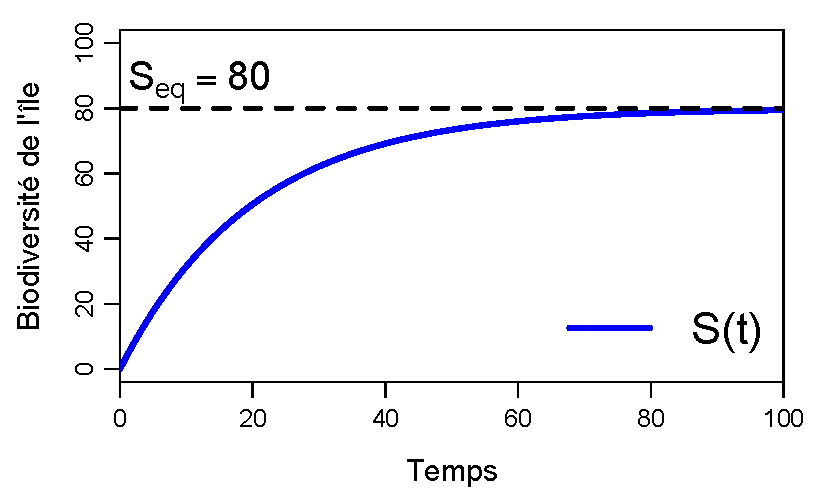
\includegraphics[width=0.9\textwidth]{annexe1/fig/figAnnI1.pdf}
\caption[Représentation graphique de la solution de l'équation différentielle]{\textbf{Représentation graphique de la solution de l'équation différentielle} \eqref{eqAnnI1} pour les conditions suivantes : $c=0.04$, $e=0.01$ et $S(0)=0$. La ligne en pointillés représente la valeur de la biodiversité $S_{eq}$ que nous obtenons à un temps infini.}
\label{figAnnI1}
\end{figure}



\section{Comment un modèle déterministe émerge-t-il de phénomènes aléatoires?}

\subsection{Modèle stochastique?}
Il est très intéressant de réaliser que l'équation \eqref{eqAnnI1}, d'apparence déterministe, renferme un modèle stochastique. "Stochastique" est un terme signifiant aléatoire, avec une part de hasard. Un modèle stochastique est donc un modèle dont l'issue contient une part de hasard; deux réalisations du modèle ne donneront donc pas nécessairement le même résultat. Pour comprendre où se cache le hasard dans le modèle que nous étudions, nous avons besoin d'objets mathématiques particuliers appartenant au domaine des probabilités : variables aléatoires et processus stochastiques (reportez-vous à l'encadré 3).

\subsection{Les objets mathématiques requis}
Comment savoir combien d’espèces sont présentes sur l’île ? Il suffit de compter 1 pour chaque espèce présente sur l’île. Nous introduisons donc $X_i$ , la variable aléatoire de présence sur l’île de l’espèce $i$ choisie parmi les $P$ espèces du continent. $X_i$ est égale à 0 si l’espèce n’est pas sur l’île et 1 si elle est sur l’île. C’est une variable aléatoire de Bernoulli (encadré 4). Ainsi, le nombre d’espèces présentes sur l’île, $S$, est égale à la somme des $X_i$. Nous allons encore plus loin en enregistrant ces valeurs au cours du temps. C'est ainsi que nous définissons le processus stochastique $X_{i,t>0}$, qui n'est autre qu'une succession de 1 et de 0 indiquant à chaque instant si oui ou non l'espèce $i$ est sur l'île. A priori, les suites $X_{i,t}$ ne sont pas prévisibles, ce qui n’exclut pas que la fonction $S$ présente, en moyenne, un comportement tout à fait régulier.

\subsection{Les briques élémentaires du modèle stochastique}
Au temps $t=0$, l'espèce $i$ n'est pas sur l'île. Pour construire la suite de son histoire, il nous faut une règle simple pour décrire l'évolution de sa présence entre deux pas de temps très proches. Le modèle de MacArthur et Wilson postule que si l'espèce considérée est sur l'île au temps $t$, elle s'éteint avec un taux $e$ ; si elle est sur le continent, elle le colonise avec un taux $c$. Pour simplifier, nous supposerons que les taux d’extinction et de colonisation sont les mêmes pour toutes les espèces. Nous donnons maintenant une signification en terme de probabilité à ces taux : $c$ est la probabilité de colonisation par unité de temps (on parle de densité du processus), $e$ est la probabilité d'extinction par unité de temps. Ainsi, $edt$ désigne la probabilité d'extinction pendant l'intervalle de temps $dt$. De même, $cdt$ est la probabilité de colonisation pendant $dt$. En faisant appel aux probabilités conditionnelles (encadré 5), en supposant $dt$ assez petit, nous différencions quatre cas:
\begin{eqnarray}
 \label{eqAnnI3a}  \forall t \in \mathbb{R}^+, ~~P(X_{i,t+dt}=1|X_{i,t}=0)&=&cdt\\
 \label{eqAnnI3b} P(X_{i,t+dt}=0|X_{i,t}=1)&=&edt \\
 \label{eqAnnI3c} P(X_{i,t+dt}=0|X_{i,t}=0)&=&(1-cdt) \\
   \label{eqAnnI3d} P(X_{i,t+dt}=1|X_{i,t}=1)&=&(1-edt)
\end{eqnarray}
Il faut comprendre la première équation ainsi : sachant que l'espèce $i$ était absente au temps $t$, la probabilité qu'elle soit sur l'île au temps $t+dt$ est égale à la probabilité qu'elle colonise l'île durant $dt$, c'est-à-dire $cdt$. Vous pourriez avancer que durant $dt$, une espèce peut coloniser, s'éteindre et re-coloniser et que nous n'en parlons pas ! Tous ces évènements sont en fait beaucoup moins probables et nous pouvons les ignorer complètement à la limite quand dt tend vers 0. Les trois autres équations s'interprètent avec un raisonnement similaire. Ces quatre équations sont les briques du modèle stochastique que nous construisons. Nous devons maintenant les assembler correctement.


\subsection{Assemblons les briques!}

L'assemblage consiste en l'utilisation de la formule des probabilités totales expliquée dans l'encadré 5. Nous pouvons en déduire la probabilité de présence de l'espèce $i$ à l'instant $t+dt$ :
\begin{eqnarray}
\label{eqAnnI4} P(X_{i,t+dt}=1)&=&P(X_{i,t+dt}=1|X_{i,t}=0)P(X_{i,t}=0)+P(X_{i,t+dt}=1|X_{i,t}=1)P(X_{i,t}=1)
\end{eqnarray}
Il s'agit d'une somme de deux termes couvrant toutes les possibilités puisque, à l'instant $t$, l'espèce $i$ était soit absente de l'île soit présente, c'est un système complet d'évènements (encadré 5). Si l'espèce $i$ était absente (premier terme) à $t$, elle sera présente à $t+dt$ si elle colonise pendant $dt$ \eqref{eqAnnI3a}. Si elle était déjà sur l'île à $t$, elle s'y maintient à condition de ne pas s'éteindre \eqref{eqAnnI3d}. En remarquant que $P(X_{i,t}=0)=1-P(X_{i,t}=1)$, nous pouvons écrire :
\begin{eqnarray}
\label{eqAnnI5a} P(X_{i,t+dt}=1)&=&cdt(1-P(X_{i,t}=1))+(1-edt)P(X_{i,t}=1)
\end{eqnarray}
Pour simplifier l'écriture, $s_{i,t}$ représente $P(X_{i,t}=1)$ :
\begin{equation}
\label{eqAnnI5b} s_{i,t+dt}=cdt(1-s_{i,t})+(1-edt)s_{i,t}
\end{equation}
Divisons par $dt$ :
\begin{eqnarray}
\label{eqAnnI5c} \frac{s_{i,t+dt}-s_{i,t}}{dt}&=&c(1-s_{i,t})-es_{i,t}
\end{eqnarray}
Nous faisons alors tendre $dt$ vers 0. Nous obtenons alors :
\begin{equation}
\label{eqAnnI5e} \frac{ds_{i}}{dt}=c(1-s_{i})-es_{i}
\end{equation}
C'est l'équation que nous avons résolu dans l'encadré 1, avec $P=1$  :
\begin{equation}
\label{eqAnnI5e} s_{i}(t)=\frac{c}{c+e} \left(1-\exp{(-(c+e)t)}\right)
\end{equation}

\subsection{Retrouvons le modèle classique}
Nous avons presque retrouvé la solution de l'équation déterministe; vous pourriez penser qu'il faut simplement multiplier par le nombre d'espèces $P$. L'idée est bonne, mais demande justification ! Nous allons effectivement considérer non pas une mais bien les $P$ espèces du continent pour lesquelles l'équation \eqref{eqAnnI5e} est valable. Nous allons alors définir un nouveau processus stochastique qui est simplement la somme des $P$ processus de présence que nous supposons indépendants $X_{i,t>0}$, $Y_t>0=X_{1,t>0}+X_{2,t>0}+....X_{P,t}$. Le problème est alors de connaître à tout instant $t$ la probabilité d'avoir un nombre donné $k$ d'espèces présentes sur l'île. À un instant donné $t$ nous faisons une somme de variable aléatoires de Bernoulli. La somme de $P$ variables de Bernoulli indépendantes est une variable aléatoire suivant une loi binomiale (encadré 5). Nous avons donc :
\begin{equation}
 \forall t \in \mathbb{R}^+, ~~\label{eqAnnI6a} P(Y_t=k)=\binom{P}{k}s(t)^k(1-s(t))^{P-k}
\end{equation}
De plus, on peut démontrer les résultats suivants :
\begin{eqnarray}
 \forall t \in \mathbb{R}^+, ~~\label{eqAnnI6b} E(Y_t)&=&Ps(t) \\
 \forall t \in \mathbb{R}^+, ~~\label{eqAnnI6c} V(Y_t)&=&Ps(t)(1-s(t))
\end{eqnarray}
Grâce à ces résultats de probabilité, nous avons donc :
\begin{equation}
 \forall t \in \mathbb{R}^+, ~~\label{eqAnnI6d} E(Y_t)=P\frac{c}{c+e}(1-\exp(-(c+e)t))
\end{equation}

Nous retrouvons la solution déterministe! Ainsi, le modèle déterministe peut être considéré comme reflétant l'évolution de l'espérance des variables $Y_t$ pour $t>0$, c'est donc l'espérance du processus stochastique. Nous pouvons alors simuler le modèle stochastique grâce au modèle déterministe : à chaque instant $t$, il suffit de simuler une loi binomiale de paramètres $P$ et $E(Y_t)$. Regardez la figure \ref{figAnnI2}, il y a des différences fondamentales entre les deux approches. Le modèle déterministe donnera des valeurs continues et, pour des paramètres donnés, toujours le même résultat. De son côté, le modèle stochastique livrera des valeurs discrètes. De plus, deux simulations du modèle aléatoire ne donneront pas nécessairement les mêmes courbes.

\begin{figure}[h!]
\centering
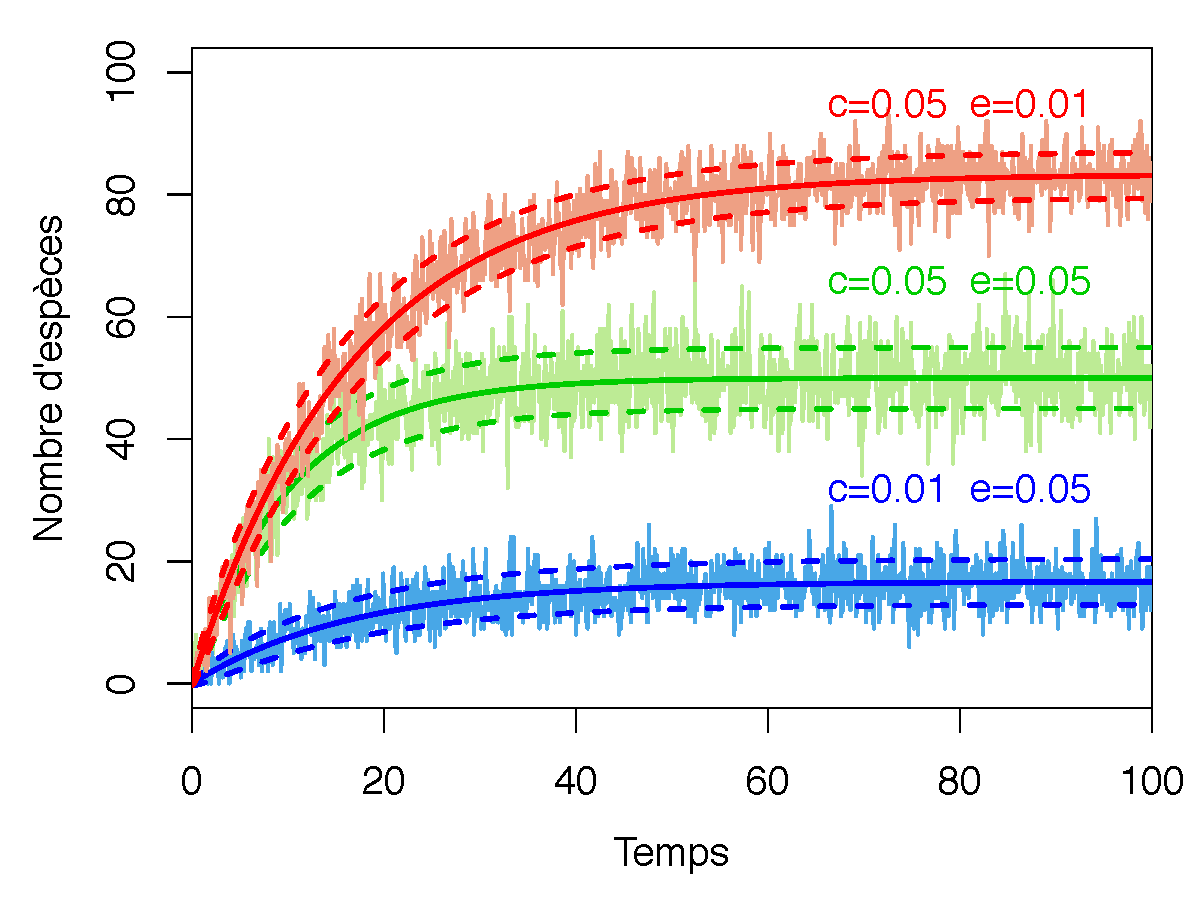
\includegraphics[width=0.9\textwidth]{annexe1/fig/figAnnI2.pdf}
\caption[Dynamique de la biodiversité de trois zones protégées]{\textbf{Dynamique de la biodiversité de trois zones protégées}. Les caractéristiques de la zone protégée sont données par les valeurs de $c$ et $e$. Les symboles rouges sont relatifs à une zone protégée de grande taille et facilement accessible, en vert, ils font référence à une petite zone facilement accessible ; enfin, en bleu, sont présentées les résultats pour une petite zone difficilement accessible. Les courbes striées en couleurs pastelles sont les réalisations du modèle stochastique. Les courbes en traits pleins, font référence au modèle déterministe qui est également la moyenne du modèle stochastique. Enfin, les courbes en pointillés représentent la moyenne du modèle stochastique plus ou moins l'écart type.}
\label{figAnnI2}
\end{figure}



\section{Applications et perspectives}

Bien que datant du milieu des années 1960, le modèle de MacArthur et Wilson demeure très précieux, notamment pour étudier les habitats fragmentés (des îles!) et prendre des décisions relatives à la conservation des espèces. Prenons un exemple : vous êtes le gestionnaire d'une nouvelle zone protégée que nous assimilerons à une île. Cette zone a longtemps été exploitée par l'homme de sorte qu'au temps $t=0$ le nombre d'espèces est $S=0$. Dans la région, la richesse en espèces est de $P=100$, c'est-à-dire que vous pouvez rencontrer jusqu'à 100 espèces dans votre aire de gestion. À la suite de MacArthur et Wilson, nous allons supposer que la valeur du taux de colonisation $c$ dépend de la difficulté d'accès. De plus, la survie d'une espèce sur cette zone dépend de sa superficie : ainsi plus l'aire de conservation est grande, moins les espèces s'éteignent ; $e$ est donc plus faible pour les grandes aires de protection. Prenons trois situations :
\begin{itemize}
\item Grande zone et accès aisé : e=0.01 et c=0.05
\item Petite zone et accès aisé : e=0.05 et c=0.05
\item Petite zone et accès délicat : e=0.05 et c=0.01
\end{itemize}
Pour mettre en place un suivi et savoir comment se comporte votre réserve, il faut avoir une idée de la dynamique attendue ! Ce que nous permet le modèle étudié, que nous simulons pour les trois situations, avec les deux approches du modèle. Les résultats sont donnés par la figure 1. Cette simple démarche vous permet d'estimer l'évolution de la biodiversité au sein de votre réserve. La paramétrisation est plus compliquée dans les faits, mais l'idée est très utilisée pour apprécier la santé des réserves naturelles.


Dans cet exemple, le modèle stochastique n'a finalement que peu d'intérêt. Il est cependant très utile si vous êtes intéressé par la variance du modèle (que nous obtenons avec l'équation \eqref{eqAnnI6c}). C'est aussi un bon point de départ pour les démarches statistiques, indispensables pour le suivi de votre réserve. De plus, l'approche stochastique révèle toute sa force pour enrichir le modèle. En partant de l'équation \eqref{eqAnnI1}, si vous souhaitiez introduire un effet des espèces les unes sur les autres (les interactions entre espèces), vous auriez quelques difficultés. Avec le travail réalisé ici vous pouvez trouver et surtout justifier des approches fertiles en réfléchissant en terme de probabilité. Ces approches pourraient vous amener à résoudre des systèmes d'équations différentielles déterministes un peu plus compliqués !


\newpage

\setlength{\columnsep}{1cm}
\begin{minipage}{0.9\linewidth}
\textbf{Encadré 1 : la Biogéographie} \\
	La biogéographie est la science qui s'interroge sur les causes de l'agencement spatial des espèces à la surface de notre planète. Comment, par exemple, pouvons-nous expliquer la répartition et les différences entre les grands biomes terrestres? Le premier élément de réponse est l'implication des facteurs climatiques. La température, l'humidité, les précipitations sont autant de variables qui contraignent les conditions d'existence des espèces qui composent et modèlent les paysages terrestres. C'est avec ces contraintes que les écologues élaborent des modèles dits "bioclimatiques" afin de décrire l'évolution de la biodiversité avec les contraintes climatiques de demain. Cependant, les facteurs qui expliquent la distribution des espèces ne sont pas toujours climatiques, les causes sont multiples. Les mouvements des espèces et leurs histoires évolutives sont ainsi des moteurs fondamentaux en biogéographie. Les capacités de dispersion des espèces leur donnent accès à de nouveaux territoires qui, avec le temps peut-être, les verront disparaître. C'est ainsi qu'un territoire voit sa composition en espèces évoluer, avec l'arrivée de nouvelles espèces et l'extinction d'autres. C'est autour de cette idée majeure que s'articule le modèle présenté.
\end{minipage}
\vspace{2cm}

\setlength{\columnsep}{1cm}
 \begin{minipage}{0.9\linewidth}
 \begin{multicols}{2}
 \textbf{Encadré 2} \\
 Il est facile de vérifier que la solution générale de l’équation homogène :
 \begin{equation}
\nonumber  \frac{dS}{dt}=-(c+e)S
\end{equation}
est donnée par :
 \begin{equation}
\nonumber \forall t \in \mathbb{R}^+,~ S(t)=C\exp(-(c+e)t)
\end{equation}
où $C$ est une constante, la solution de l’équation non homogène est alors de la forme :
 \begin{equation}
\nonumber S(t)=f(t) \exp(-(c+e)t)
\end{equation}
En remplaçant dans l’équation différentielle on obtient :
 \begin{equation}
\nonumber f’(t) \exp(-(c+e)t)= cP
\end{equation}
ce qui nous donne :
 \begin{equation}
\nonumber f’(t)= cP \exp((c+e)t)
\end{equation}
En intégrant on obtient :
 \begin{equation}
\nonumber f(t)= P\frac{c}{c+e} \exp({(c+e)t}) + K
\end{equation}
où $K$ est une constante arbitraire.
 \begin{equation}
\nonumber S(t)= P\frac{c}{c+e} + K\exp(-(c+e)t)
\end{equation}
Avec $S(0)=0$, $K=-P\frac{c}{c+e}$, nous obtenons donc :
 \begin{equation}
\nonumber S(t)= P\frac{c}{c+e} (1-\exp(-(c+e)t))
\end{equation}
\end{multicols}
 \end{minipage}
\vspace{2cm}

\setlength{\columnsep}{1cm}
 \begin{minipage}{0.9\linewidth}
\textbf{Encadré 3} \\
Les \textbf{variables aléatoires} sont des fonctions définies sur l’ensemble des résultats possibles d’un événement aléatoire. Comme le résultat de l’événement est aléatoire, on associe à chaque valeur de la variable sa probabilité, de sorte que la somme des probabilités sur l'ensemble des valeurs possibles soit égale à 1. Dans notre exemple, $X_i$ est une variable aléatoire, 0 et 1 sont ses valeurs, et nous nous intéressons à leur probabilité $P(X_i=1)$ et $P(X_i=0)$ avec $P(X_i=1)+P(X_i=0)=1$. \\
Les \textbf{processus aléatoires ou stochastiques} sont des collections de variables aléatoires indexées par le temps $t$, c'est-à-dire ordonnées. Dans notre exemple, l'indexation est faite selon le temps $t$. Nous suivons ainsi l'évolution de $X_i$ au cours du temps d'où la notation $X_{i,t>0}$. Attention ! $X_{i,t>0}$ est un processus aléatoire mais $X_{i,t}$ est l'une des variables aléatoires du processus.
 \end{minipage}
\vspace{2cm}

\setlength{\columnsep}{1cm}
 \begin{minipage}{0.9\linewidth}
 \textbf{Encadré 4} \\
Une variable aléatoire $X$ suit un \textbf{schéma de Bernoulli} lorsqu'elle prend uniquement deux valeurs 0 ou 1. Si nous notons $p=P(X=1)$, nous avons :
\begin{itemize}
\item $P(X=0)=1-p$
\item $E(X)=p$
\item $V(X)=p(1-p)$
\end{itemize}
$X$ est alors une variable aléatoire de Bernoulli de paramètre $p$. \\
Une variable aléatoire $X$ suit une \textbf{loi Binomiale} de paramètres $n\in\mathbb{N}$ et $p\in[0,1]$ lorsqu'elle est la somme de $n$ variables de Bernoulli indépendantes de paramètre $p$. On peut alors montrer les résultats suivants :
\begin{itemize}
\item $\forall k \leq n,~ P(X=k)=\binom{n}{k}p^k(1-p)^{n-k}$
\item $E(X)=np$
\item $V(X)=np(1-p)$
\end{itemize}
 \end{minipage}
\\  \\  \\


\begin{figure}[h!]
\centering
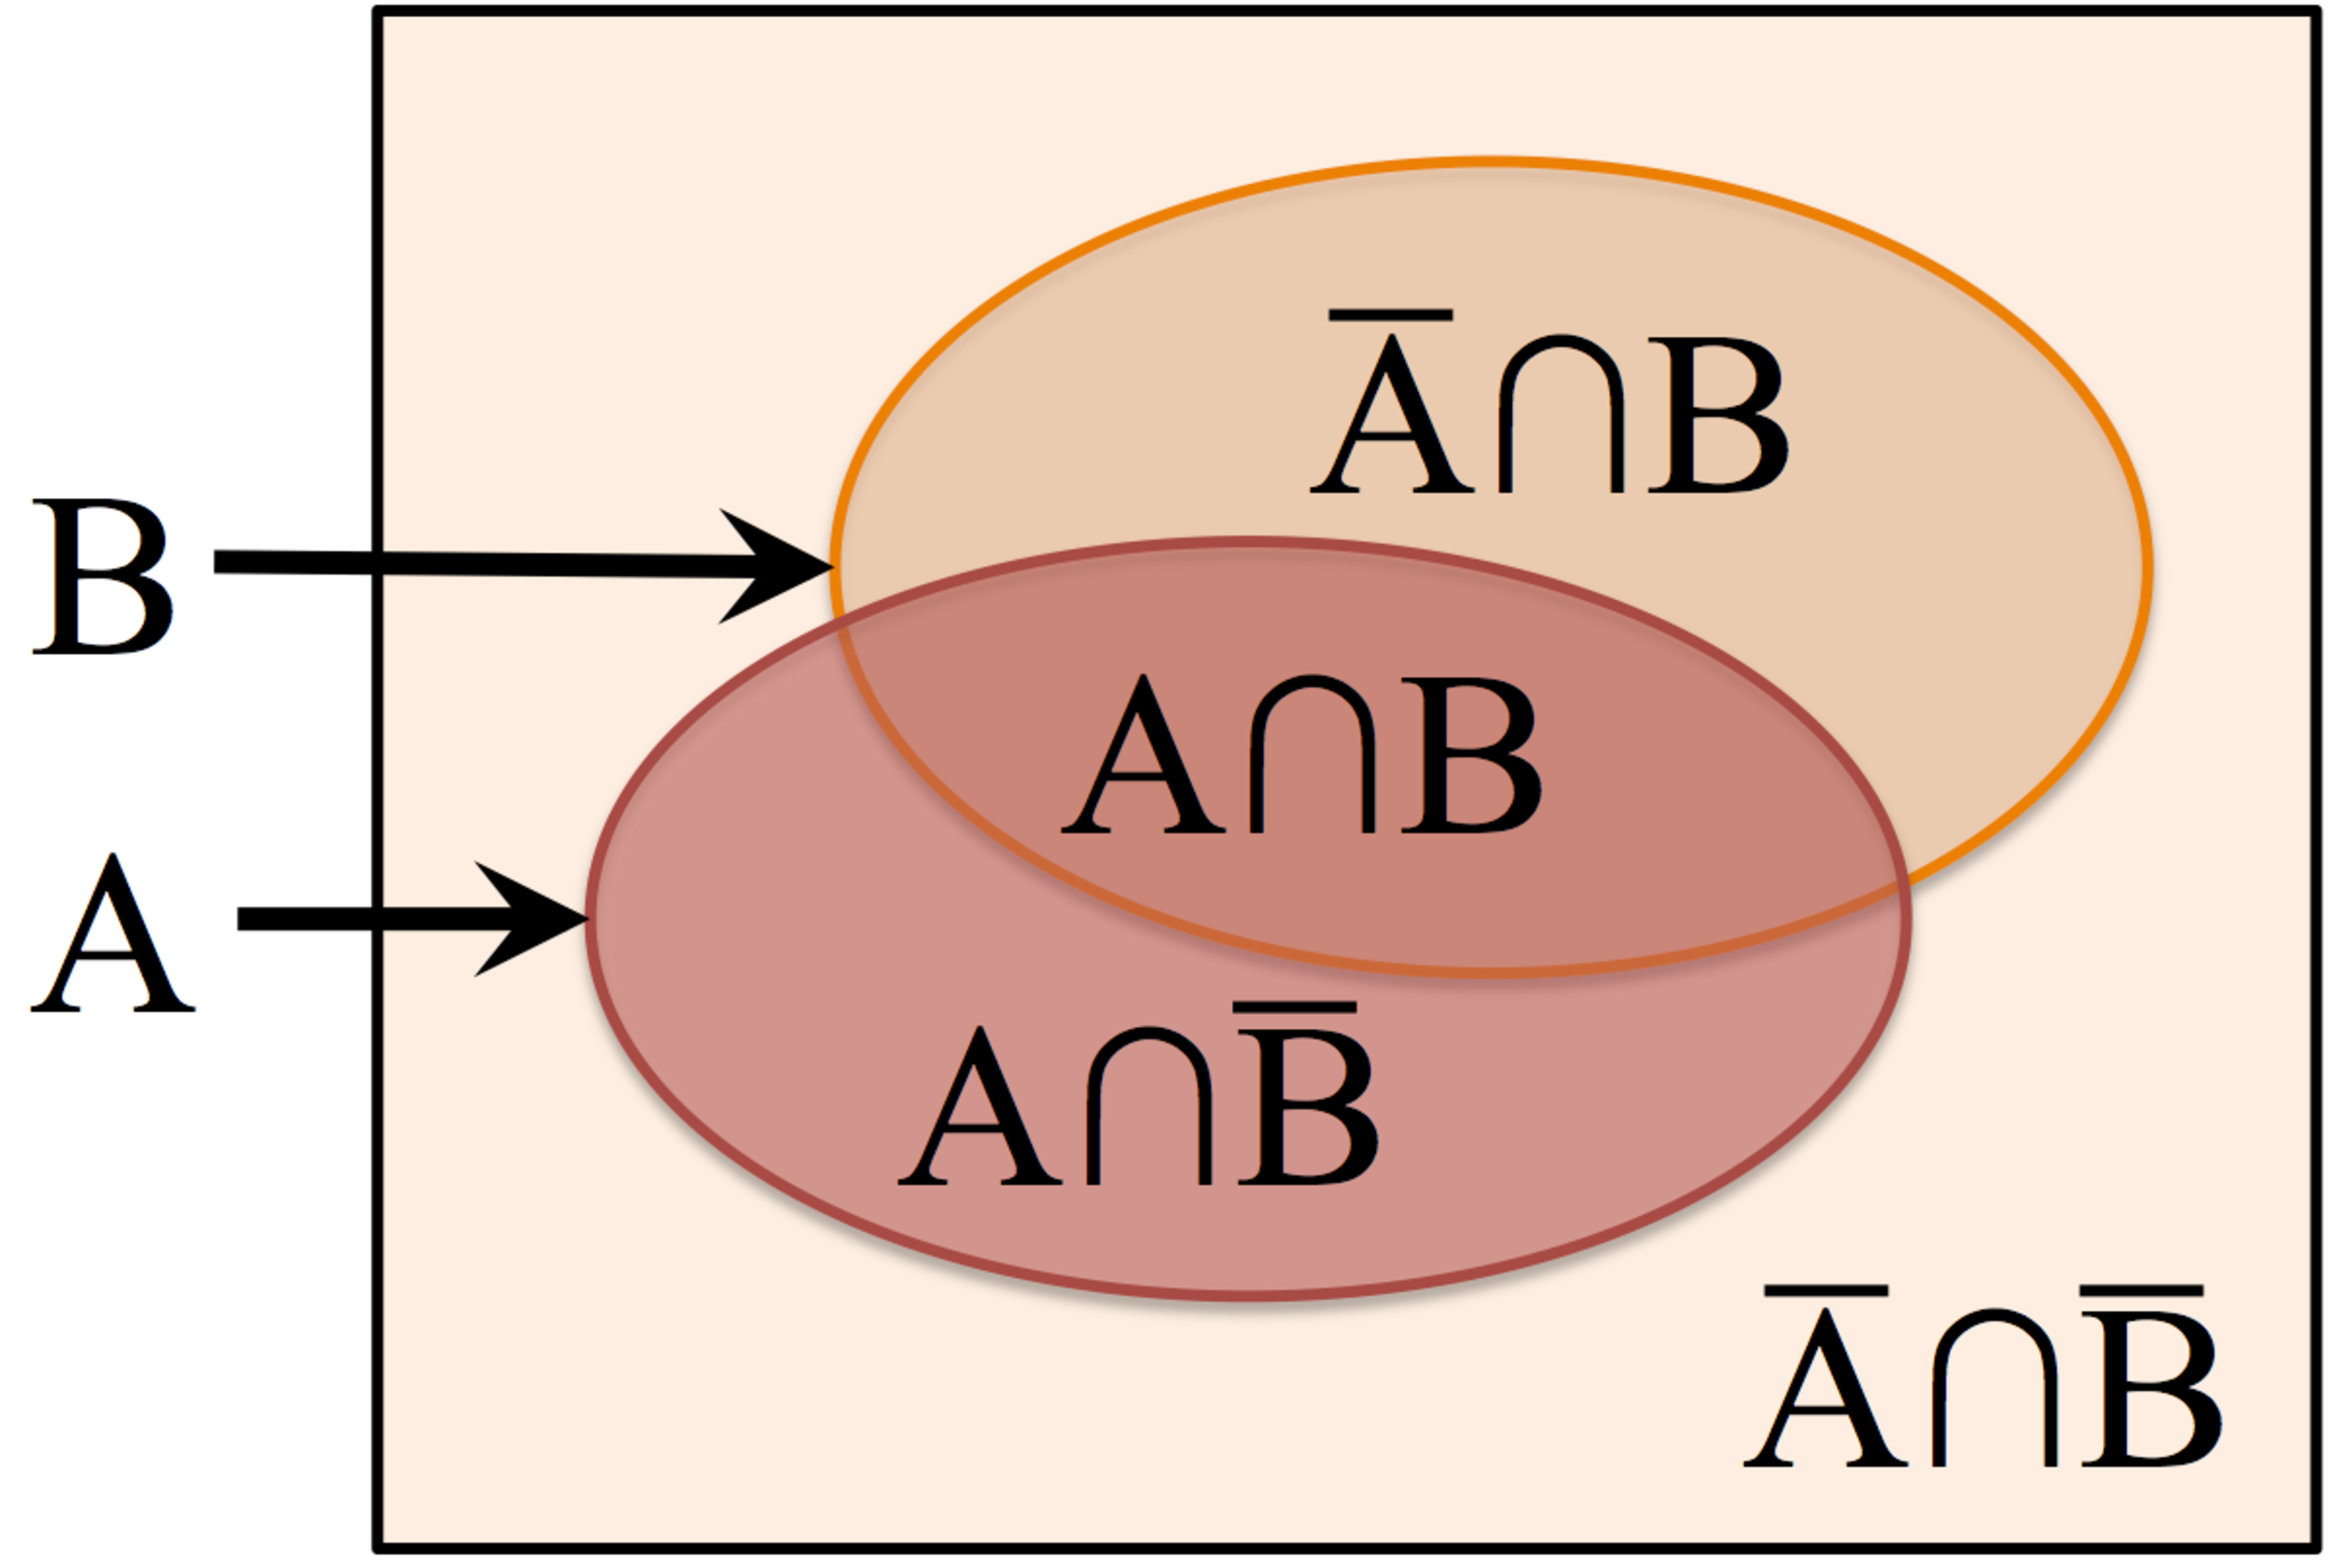
\includegraphics[width=0.95\textwidth]{annexe1/fig/figAnnI3.pdf}
\caption[Représentation de la formule des probabilités totales.]{\textbf{Représentation de la formule des probabilités totales}. $A$ et $B$ sont deux événements. La probabilité de A peut être décrite comme la somme de l'intersection avec $B$ et $\bar B$ qui constituent un système complet d'évènements.}
\label{dess1}
\end{figure}

\setlength{\columnsep}{1cm}
\begin{minipage}{0.9\linewidth}
\textbf{Encadré 5} \\
Une \textbf{probabilité conditionnelle}, est une probabilité qu'un évènement se réalise à condition qu'un autre soit déjà réalisé. Soit deux évènements $A$ et $B$, la probabilité de $A$ sachant $B$, notée ici $P(A|B)$ est la probabilité que $A$ se réalise lorsque B est réalisé. \\
Un \textbf{système complet d'évènements} est un ensemble d'événements exclusifs dont la somme des probabilités est 1. Par exemple, l'évènement $B$ et son complémentaire $\bar{B}$ forme un tel système (voir figure \ref{dess1}).\\
La \textbf{formule des probabilités totales} nous donne la probabilité de réalisation d'un évènement à partir de la connaissance de probabilités conditionnelles sous réserve que l'ensemble des évènements du conditionnement forment un système complet d'évènements. Ainsi pour connaître la probabilité de $A$, nous pouvons écrire :
\begin{align*}
\begin{split}
P(A)&=P(A\cap B)+ P(A\cap\bar{B})\\
& =P(A|B)P(B)+P(A|\bar{B})P(\bar{B}).\end{split} \end{align*}

\end{minipage}
